\documentclass[journal]{IEEEtran}
\usepackage[a5paper, margin=10mm, onecolumn]{geometry}
\usepackage{tfrupee}
\usepackage{amsmath, amssymb, amsfonts, amsthm}
\usepackage{algorithmic}
\usepackage{graphicx}
\usepackage{textcomp}
\usepackage{xcolor}
\usepackage{txfonts}
\usepackage{listings}
\usepackage{enumitem}
\usepackage{mathtools}
\usepackage{gensymb}
\usepackage{comment}
\usepackage[breaklinks=true]{hyperref}
\usepackage{tkz-euclide} 
\usepackage{listings}
\usepackage[latin1]{inputenc}                                
\usepackage{color}                                            
\usepackage{array}                                            
\usepackage{longtable}                                       
\usepackage{calc}                                             
\usepackage{multirow}                                         
\usepackage{hhline}                                           
\usepackage{ifthen}                                           
\usepackage{lscape}
\newcommand{\myvec}[1]{\begin{pmatrix} #1 \end{pmatrix}}

\begin{document}

\bibliographystyle{IEEEtran}
\vspace{3cm}

\title{NCERT-10.3.4.1.2}
\author{EE24BTECH11042 - SRUJANA}
{\let\newpage\relax\maketitle}

\renewcommand{\thefigure}{\theenumi}
\renewcommand{\thetable}{\theenumi}
\setlength{\intextsep}{10pt} 

\numberwithin{equation}{enumi}
\numberwithin{figure}{enumi}
\renewcommand{\thetable}{\theenumi}

\textbf{QUESTION}:

Solve the following pair of linear equations:

\hspace{3cm}3x + 4y = 10

\hspace{3cm}2x - 2y = 2

\textbf{Theoretical Solution}:\\

\begin{align}
    x &= 1 + y \tag{1} \\
    3(1 + y) + 4y &= 10 \tag{2} \\
    7y &= 7 \tag{3} \\
    y &= 1, \quad x = 2 \tag{4}
\end{align}

\textbf{LU Decomposition Method}\\

LU decomposition is a mathematical method used to solve systems of linear equations \(Ax = b\), where \(A\) is a square matrix, \(x\) is an unknown vector, and \(b\) is a constant vector. It is especially useful for efficiently solving multiple systems of equations with the same coefficient matrix.

In this method, we decompose \(A\) into the product of two matrices \(L\) and \(U\), where \(L\) is a lower triangular matrix and \(U\) is an upper triangular matrix.

This decomposition allows us to solve the system in two steps:
\begin{enumerate}
    \item Solve \(Ly = b\)
    \item Solve \(Ux = y\)
\end{enumerate}

Given the system of equations:
\[
3x + 4y = 10 \tag{5}
\]
\[
2x - 2y = 2 \tag{6}
\]

We represent the system in matrix form:
\[
A = \begin{bmatrix} 3 & 4 \\ 2 & -2 \end{bmatrix}, \quad b = \begin{bmatrix} 10 \\ 2 \end{bmatrix} \tag{7}
\]

\textbf{Step 1: LU Decomposition}
\begin{align}
    A &= LU \tag{8} \\
    L &= \begin{bmatrix} 1 & 0 \\ l_{21} & 1 \end{bmatrix}, \quad U = \begin{bmatrix} u_{11} & u_{12} \\ 0 & u_{22} \end{bmatrix} \tag{9}
\end{align}

From \(LU = A\):
\begin{align}
    u_{11} &= 3, \quad u_{12} = 4 \tag{10} \\
    l_{21} &= \frac{2}{3}, \quad u_{22} = -2 - \frac{2}{3} \times 4 = -\frac{14}{3} \tag{11}
\end{align}

Thus:
\[
L = \begin{bmatrix} 1 & 0 \\ \frac{2}{3} & 1 \end{bmatrix}, \quad U = \begin{bmatrix} 3 & 4 \\ 0 & -\frac{14}{3} \end{bmatrix} \tag{12}
\]

\textbf{Step 2: Solve \(Ly = b\)}
\[
\begin{bmatrix} 1 & 0 \\ \frac{2}{3} & 1 \end{bmatrix} \begin{bmatrix} y_1 \\ y_2 \end{bmatrix} = \begin{bmatrix} 10 \\ 2 \end{bmatrix} \tag{13}
\]

\begin{align}
    y_1 &= 10 \tag{14} \\
    \frac{2}{3}y_1 + y_2 &= 2 \quad \Rightarrow \quad y_2 = 2 - \frac{2}{3} \times 10 = -\frac{14}{3} \tag{15}
\end{align}

\textbf{Step 3: Solve \(Ux = y\)}
\[
\begin{bmatrix} 3 & 4 \\ 0 & -\frac{14}{3} \end{bmatrix} \begin{bmatrix} x_1 \\ x_2 \end{bmatrix} = \begin{bmatrix} 10 \\ -\frac{14}{3} \end{bmatrix} \tag{16}
\]

\begin{align}
    3x_1 + 4x_2 &= 10 \tag{17} \\
    -\frac{14}{3}x_2 &= -\frac{14}{3} \quad \Rightarrow \quad x_2 = 1 \tag{18} \\
    3x_1 &= 6 \quad \Rightarrow \quad x_1 = 2 \tag{19}
\end{align}

\textbf{Final Solution}
\[
x = \begin{bmatrix} 2 \\ 1 \end{bmatrix} \tag{20}
\]

\section*{LU Decomposition using Doolittle's algorithm}
The LU decomposition can be efficiently compted using Doolittle's algorithm. This method generates the matrices \( L \) (lower triangular) and \( U \) (upper triangular) such that \( A = LU \). The elements of these matrices are calculated as follows: \\
Elements of the \( U \) Matrix:  \\
For each column \( j \):
\begin{align}
	U_{ij} &= A_{ij} \quad \text{if } i = 0, \\
	U_{ij} &= A_{ij} - \sum_{k=0}^{i-1} L_{ik} U_{kj} \quad \text{if } i > 0.
\end{align}
Elements of the \( L \) Matrix: \\
For each row \( i \):
\begin{align}
	L_{ij} &= \frac{A_{ij}}{U_{jj}} \quad \text{if } j = 0, \\
	L_{ij} &= \frac{A_{ij} - \sum_{k=0}^{j-1} L_{ik} U_{kj}}{U_{jj}} \quad \text{if } j > 0.
\end{align}


\begin{figure}[h!]
   \centering
   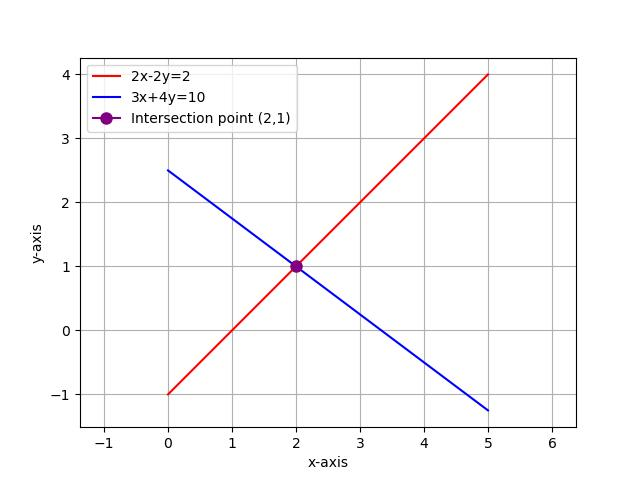
\includegraphics[width=\columnwidth]{fig/combined_fig.jpg}
\end{figure}


\end{document}
